%------------------------------------------------------------
% Pakete
%------------------------------------------------------------
\documentclass[12pt, parskip=half]{scrartcl}% Schriftgröße 12pt, Abstand zwischen Absätzen
\usepackage[utf8x]{inputenc}			%Wird für die direkte Eingabe von Umlauten gebraucht.
\usepackage[ngerman]{babel}				%Eine Sammlung von verschieden Sprachen, und ermöglicht für diese Sprachen die automatische Worttrennung und die ändert die Bezeichnungen in die jeweilige Sprache.
\usepackage[T1]{fontenc}				%westeuropäische Schriftkodierung verwenden
\usepackage{lmodern}					%andere Schriftart
\usepackage[babel=once]{csquotes}%Befleh \enquote für Anführungszeichen
\usepackage{amsmath, amssymb, amstext}	%Mathematische Erweiterungen
\usepackage[breaklinks]{hyperref}
\usepackage{graphicx} 					%Das Standardpaket zum Einbinden von Bildern / Grafiken. Kann auch zum Einbinden von PDF Seiten genutzt werden. 
\usepackage{pdfpages}					%Das Paket zum einbinden von PDF Dateien in ein LaTeX Dokument, wobei bei der Beamer Class das Paket graphicx dafür verwendet werden sollte.
\usepackage{setspace} 					%Damit kann der Zeilenabstand einfach geänderter zum 1.5 facher oder 2 facher Zeilenabstand.
\usepackage{xcolor} 					%Ermöglicht das Nutzen von Farben zum Beispiel farbige Schrift.
\usepackage{tikz} 						%Ist zwar dem Namen nach kein Programm zum Zeichen tikz - "tikz ist kein Zeichenprogramm". Es lassen sich damit dennoch schöne 	Bilder machen. Im Zusammenspiel mit gnuplot lassen sich auch Funktionen plotten.
\usepackage[section]{placeins}			%placeins ist ein Paket, welches verhindert, dass Floats hinter dem Befehl \FloatBarrier erscheint.
										%Der Standard Befehl \section{} wird so verändert, dass er immer einen \FloatBarrier am Anfang mit sich trägt.
\usepackage{geometry}					%Ermöglicht die einfacherer Einstellung der Seitenränder
\usepackage{listings}					%zum einbinden von Quelltext
\usepackage{todonotes}
\usepackage{caption} 					%Zum Ändern der Beschriftung von Tabellen und Bildern.
\usepackage{ulem}
\usepackage{verbatim}					%Zum erstellen von mehrzeiligen Kommentaren
%------------------------------------------------------------
% Dokumenteneinstellung
%------------------------------------------------------------
\geometry{a4paper, top=25mm, left=20mm, right=20mm, bottom=30mm, headsep=10mm, footskip=12mm}
\onehalfspacing							%Zeilenabstand 1.5
%\par\bigskip 
%\parindent=0pt							%verhindert das Einrücken
\lstset
{
	language=C,
	basicstyle=\tiny,
	keywordstyle=\color{blue}\ttfamily,
	stringstyle=\color{red}\ttfamily,
	commentstyle=\color{green}\ttfamily,
	showstringspaces=false,
	morecomment=[l][\color{magenta}]{\#}
}

%------------------------------------------------------------
% Deckblatt und Inhaltsverzeichnis
%------------------------------------------------------------
\begin{document}
	
%\input{./Deckblatt/Deckblatt.tex}

\begin{titlepage}
	\vspace*{2.5cm}
	\begin{center}
		
		{\LARGE Modellbasierter Entwurf} \\ [1cm]
		\rule{\textwidth}{1pt}\\ [0.5cm]
		\textbf{\Huge {Neuronale Netze}}
		\rule{\textwidth}{1pt}\\[2cm]
		
		\begin{figure}[h]
			\centering
			
\includegraphics[width=0.2\linewidth]{./Bilder/Deckblatt/Beuth-Logo_single}
			\label{fig:Beuth-Logo_single}
		\end{figure}
		
		
		\bigskip 
		{\large BEUTH HOCHSCHULE FÜR TECHNIK BERLIN} \\
		University of Applied Sciences \\ 
		Fachbereich VI \\
		Technische Informatik\\ [5cm]
		
		\vfill	
		\large
		\begin{tabular}{|c|c|} %Teilnehmer
			\hline
			\textbf{Teilnehmer} & \textbf{Matrikelnummer} \\ 
			\hline 
			Bryan Scheffner & 888777 \\ 
			%\hline 
			Toni Reichel & 897991 \\ 
			\hline 
		\end{tabular}
		\normalsize
	\end{center}
\end{titlepage}

\tableofcontents
\setcounter{page}{2}
\newpage
		
%------------------------------------------------------------
% ab hier beginnt das eigentliche Dokument
%------------------------------------------------------------
\newcommand{\faq}[2]{%
	{\scshape Frage:} \normalfont\sffamily\textsf{#1}\par
	\noindent{\scshape Antwort:} #2
}

\section{Einleitung}

\subsection{Motivation neuronaler Netze}
Heutzutage findet man in nahezu allen Bereichen des Lebens Programme vor, sei es in Zahnbürsten, Autos oder in Robotern am Fließband. Mithilfe von Programmen sollen also sich wiederholende Aufgaben vereinfacht oder automatisiert werden. Dafür werden die Programme mit prozedurale oder objektorientierte Methoden entwickelt. Bevor mit der Programmierung angefangen werden kann, muss zuerst ein Modell des Problems entworfen werden. Bei einfachen Anwendungen, wie zum Beispiel einer Zahnbürste ist es recht einfach. Möchte man allerdings ein Modell für eine Mustererkennung 

\subsection{Das menschliche Nervensystem}
Das menschliche Gehirn besteht aus etwa 86 Milliarden Nervenzellen, auch Neuronen genannt, die zum Zentralnervensystem miteinander verschaltet sind (im folgendem Nervensystem). Nervenzellen im Gehirn sind hochspezialisierte Zellen, die sich im Gegensatz zu einfacheren Zellen nicht teilbar sind. Das bedeutet, dass sich das Nervensystem nicht über Zellteilung regenerieren kann. Allerdings schafft es das Gehirn durch die Verknüpfung anderer Nervenzellen den Defekt teilweise oder komplett auszugleichen. Jede Nervenzelle kann mit bis zu 10.000 anderen Nervenzellen in Verbindung stehen. 

Jede Nervenzelle ist zwar im Grundaufbau gleich, kann aber unterschiedliche Formen und Größen haben. Das liegt unter anderem daran, dass sich Nervenzellen weiter spezialisieren. So können die einen Nervenzellen eher für motorische und die anderen eher für sensorische Aufgaben bestimmt sein. Dadurch erreichen Nervenzellen unterschiedliche Geschwindigkeiten, wie sie Informationen an andere Nervenzellen weitergeben. Der Informationsfluss ist dabei immer in die gleiche Richtung. In Abbildung \ref{AufbauNeuron} ist der Aufbau einer Nervenzelle dargestellt.

\begin{figure}[hbt]
	\centering
	\includegraphics[width=0.9\linewidth]{./Bilder/Aufbau_Gehirn_gehirnlernen-de}
	\caption{Aufbau Neuron}
	\label{AufbauNeuron}
\end{figure}

Der hier stark vereinfachte Aufbau einer Nervenzelle besteht aus dem Zellkörper, den Dendriten, dem Axon und den Synapsen. Der Zellkörper bildet die zentrale Einheit einer Nervenzelle und erhält seine Informationen über die Dendriten. Die Dendriten sind baumartig verzweigt und mit anderen Nervenzellen über Synapsen verbunden. Der Zellkörper bildet eine Summation über die Signale der vielen verschieden Dendriten. Dabei kann jedes Dendrit eine erregende oder hemmende Wirkung auf den Zellkörper haben. Bei ausreichender Stärke leitet der Zellkörper das Signal weiter. Wenn eine Erregungsweiterleitung stattfindet, wird das Signal über das Axon und Synapsen an die nächste Nervenzelle weitergeleitet. Ein Axon hat einen Durchmesser von 0,002 - 0,01 Millimetern und kann bis zu einem Meter lang sein. Umso dicker ein Axon ist, desto schneller findet auch die Weiterleitung statt. Jede Nervenzelle kann nur über ihre Synapsen mit anderen Nervenzellen kommunizieren. Dafür hat jede Nervenzelle bis zu 10.000, in manchen Extremfälle sogar mehr als 100.000 Synapsen. Synapsen kommunizieren untereinander mit chemischen oder elektrischen Signalen. Wobei elektrische in chemische und chemische in elektrische Signale umgewandelt werden. In der Regel kommunizieren Synapsen über chemische Signale. Der Grund dafür ist, dass Synapsen meisten keinen direkten Kontakt zueinander haben, sondern ein kleiner Abstand von 20 bis 50 Nanometern bleibt. Bei elektrischen Synapsen ist der Abstand so nah, dass über eine kleine Brücke (gap junction) kommuniziert wird. Dabei kann das Signal schneller weitergeleitet werden.

Das Nervensystem ist ein großes Netz aus sehr vielen Nervenzellen, die unterschiedlich stark miteinander verbunden sind und unterschiedlich schnell Signale weiterleiten. Wenn eine Nervenzelle ein Signal auslöst, weil eine gewisse Schwelle überschritten wurde spricht man auch davon, dass das Aktionspotenzial erreicht wurde. Das Aktionspotenzial kann nur erreicht werden, wenn vorher genügend vorgeschaltete Nervenzellen ein Signal gesendet haben. Der Anfang einer Verkettung von Nervenzellen kann zum Beispiel über sehen, schmecken, spüren oder ähnliches stattfinden. Wird ein Aktionspotenzial in den dafür verantwortlichen Nervenzellen erreicht, werden sie wieder Signale an andere Nervenzellen senden. Am Ende kann das Signal bei Nervenzellen ankommen, die für eine Bewegung verantwortlich sind, wie zum Beispiel eine Gehbewegung. Das ist ein sehr stark vereinfachtes Beispiel und soll nur dazu dienen die Mechanismen eines Nervensystems zu verstehen.

Dieser Text Falls im Text in diesem Abschnitt nicht anders angegeben sind über die Quellen \cite{dasgehirn.info} und \cite{gehirnlernen.de} zu finden.
%\section{Labor 1}
In \cite[S. 12]{Mazzetti1996} der Laborübung sollen erste Erfahrungen mit der Vivado IDE und dem Xilinx SDK gemacht werden. Zunächst werden in der Vivado IDE die Verbindung des Prozessors zur Peripherie hergestellt, um anschließend mit dem SDK ein Programm schreiben zu können, was es erlaubt LEDs auf dem Zedboard blinken zu lassen.

Für diese Laborübung waren folgende Fragen als Vorbereitung zu bearbeiten:

\faq{Hat der ARM Prozessor Memory Mapped oder Isolated IO?}
    {Bei Memory Mapped werden die Register der Peripheriegeräte innerhalb des gewöhnlichen Adressraumes abgebildet und als solche angesteuert. Beim Isolated IO verwendet man hingegen einen isolierten Adressraum. Bei einem ARM Prozessor wird Memory Mapped verwendet. Das kann zum Beispiel im Dokument UG585 in der Tabelle 4-1 erkannt werden. Dort werden alle Adressen dargestellt, die sich im PS befinden.}

\subsection{Aufgabe 1}

In der ersten Aufgabe haben wir ein Block Design in der Vivado IDE erstellt. Hier gibt es eine Abweichung zur Aufgabenstellung. Wir verwenden in all unseren Laboren das Zybo-Board von Digilent, welches nur 4 LEDs besitzt. Aus Diesem Grund sind an dem AXI-GPIO0-Block nur vier LEDs angeschlossen. Im Bild \ref{Labor1_Aufgabe1_Bild1} ist das komplette Block Design dargestellt. Die Konfiguration des FPGAs ermöglicht es die LEDs über die Programmbale Logic (PL) und das Processing System (PS) anzusprechen. Dafür werden 435 LUTs, 60 LUTRAMs, 613 Flip Flops, ein BUFG und vier Inputs/Outputs verwendet.

\begin{figure}[hbt]
	\centering
	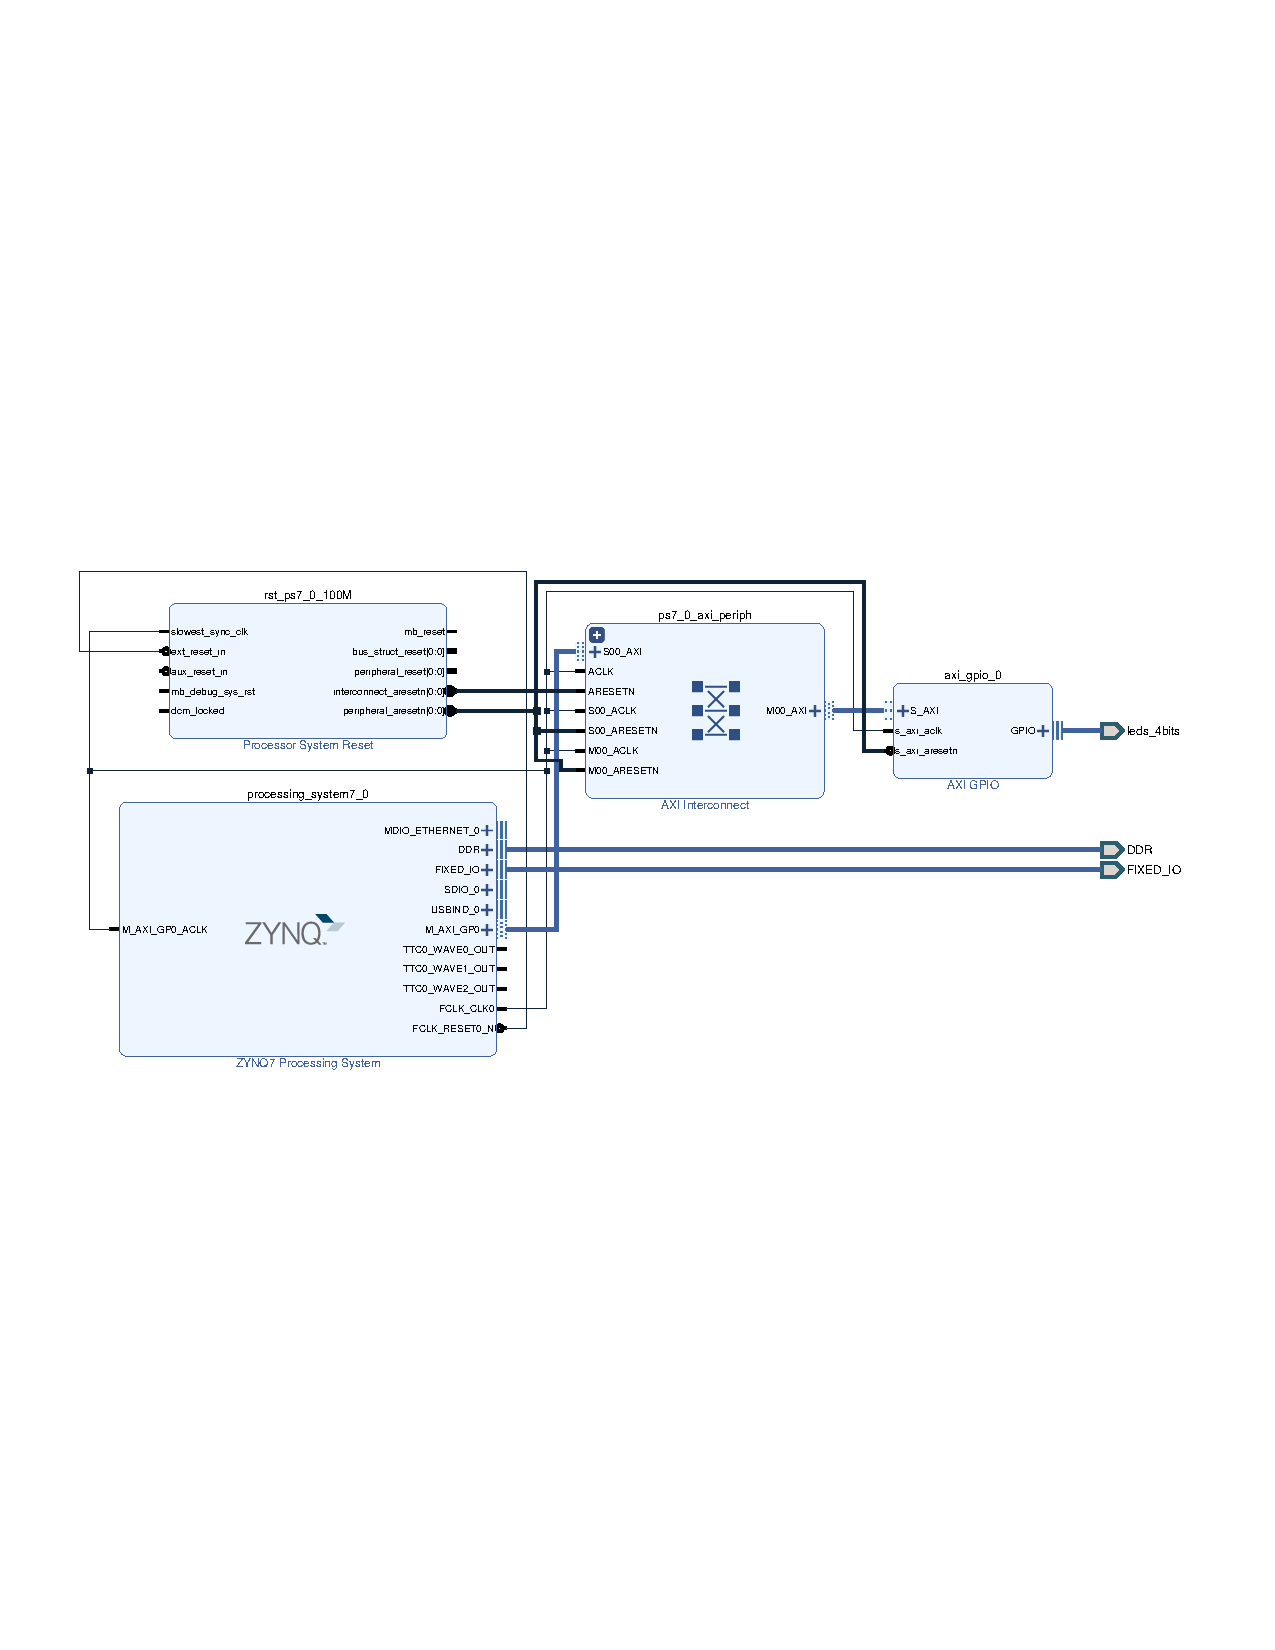
\includegraphics[trim = 10mm 100mm 10mm 100mm, width=0.9\linewidth]{./Bilder/Labor1_Aufgabe1_Bild1}
	\caption{LED Ansteuerung über AXI GPIO}
	\label{Labor1_Aufgabe1_Bild1}
\end{figure}

\subsection{Aufgabe 2}
In der Aufgabe 2 wird ein C-Programm geschrieben, um die LEDs über das PS zu steuern. Der Quellcode ist in der Aufgabenstellung gegeben und wurde nicht modifiziert.

In dem vorgegebenen Programm werden zuerst die GPIO initialisiert und danach geht das Programm in eine Endlosschleife. In der Schleife werden die LEDs in einem bestimmten Muster eingeschaltet und anschließend eine gewisse Zeit gewartet, bevor die Schleife mit dem invertierten Muster von vorne beginnt.

\faq{Wie funktioniert die Funktion XGpio\_DiscreteWrite}
    {Die hier zu beschreibende Funktion soll in ein Register schreiben, um GPIOs zu setzten. Zuerst wird der übergebene Pointer mit dem Typ XGpio überprüft, ob er gültig ist. Ist der Übergabeparameter kein Null-Pointer wird getestet, ob der GPIO-Port bereit ist und ein Kanal angegeben wurde. Ist alles korrekt wird der Pointer weiter an die Funktion XGpio\_WriteReg gegeben.}

\faq{Woran / Wo sieht man die Antwort von der Vorbereitung im Code?}
    {Über die Datei xil\_io.h kann direkt in einen Speicher geschrieben werden. Die Zuweisungen der Registeradressen sind in xparameters.h zu finden.}
    
\subsection{Aufgabe 3}
In der dritten Aufgabe sollen nicht nur die LEDs über GPIO , sondern auch die Schalter bzw. Knöpfe angesteuert werden. In Abbildung \ref{Labor1_Aufgabe3_Bild1} ist ein weiterer GPIO-Block mit dem Namen \textit{axi\_gpio\_0} hinzugekommen.

In Quellcode \ref{Labor1_Aufgabe3_Code1} werden erst die GPIOs konfiguriert und danach geht das Programm in eine Endlosschleife. In der Endlosschleife werden die Schalter ausgelesen und der ausgelesen Wert auf die LEDs angewendet. Am Ende folgt eine Pause, erst danach geht die Schleife von vorne los.

\begin{figure}[hbt]
	\centering
	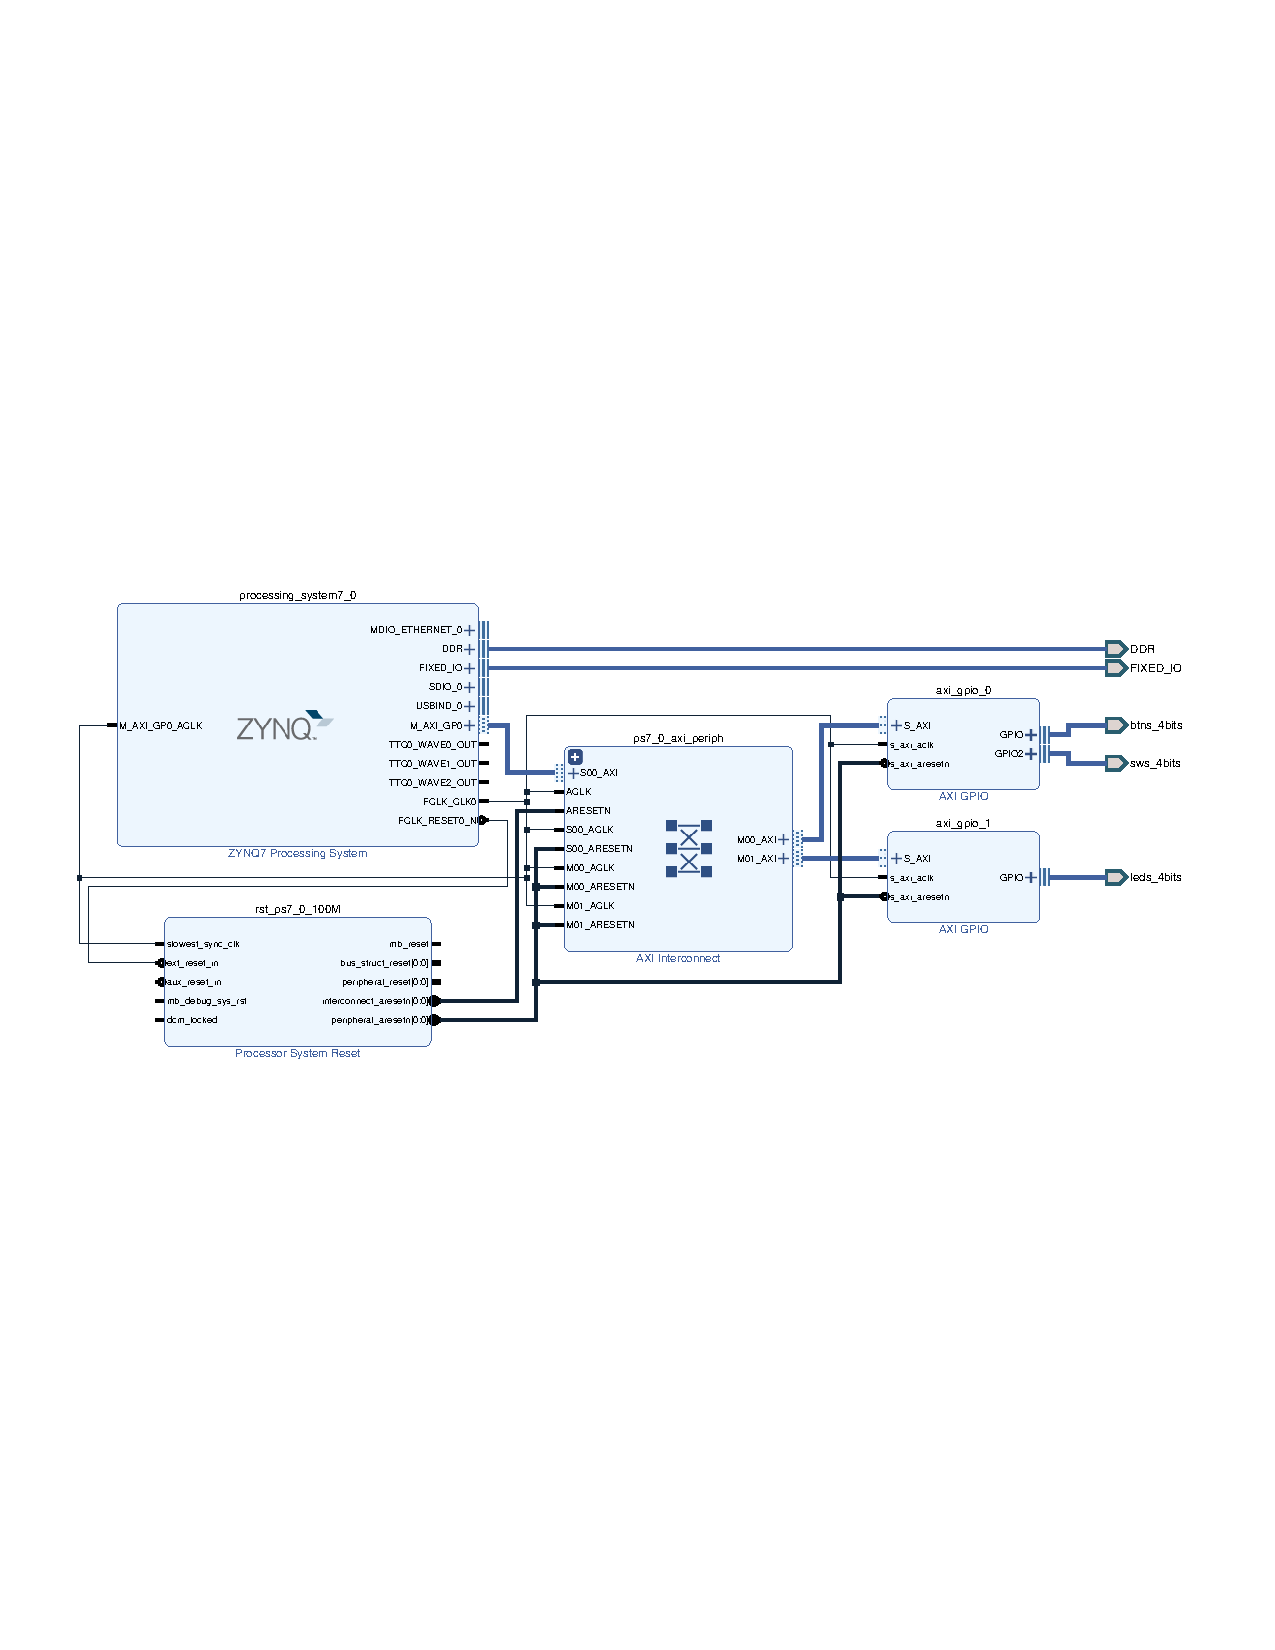
\includegraphics[trim = 10mm 100mm 10mm 100mm, width=0.9\linewidth]{./Bilder/Labor1_Aufgabe3_Bild1}
	\caption{LED Ansteuerung über AXI GPIO}
	\label{Labor1_Aufgabe3_Bild1}
\end{figure}
\FloatBarrier
\lstinputlisting[frame=single,caption=Lesen von Schaltern und Knöpfen,label=Labor1_Aufgabe3_Code1]{./Quellcode/Labor1_Aufgabe3_Code1.c}
%\input{./Laboruebung2.tex}
%\input{./Laboruebung3.tex}
%\input{./Laboruebung4.tex}

%------------------------------------------------------------
% Anhang
%------------------------------------------------------------
\newpage
\bibliographystyle{plain}
\bibliography{bibliography.bib}
%\clearpage
%\section{Anhang}
%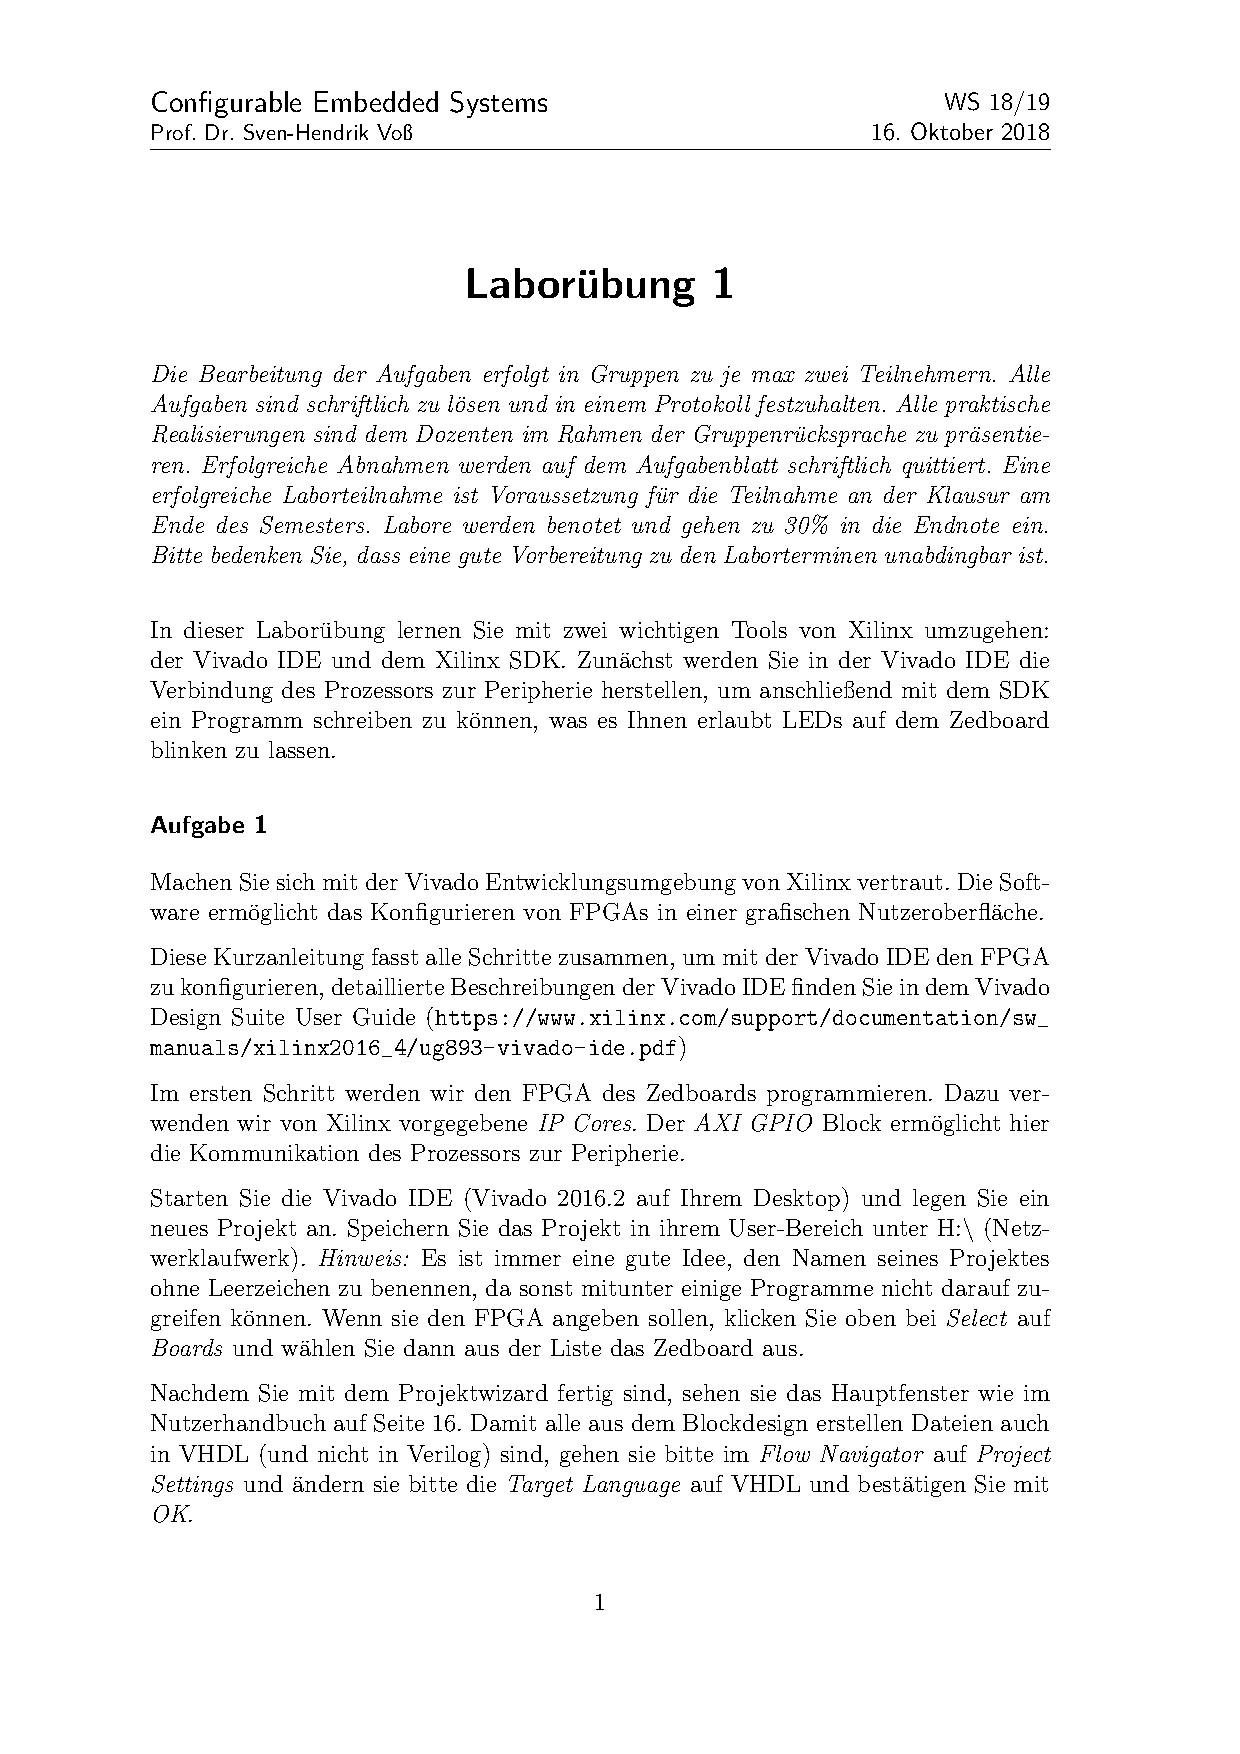
\includepdf[pages=-,frame=true,scale=0.8]{./Anhang/CES_Laboruebung_1}
%\includepdf[pages=-,frame=true,scale=0.8]{./Anhang/CES_Laboruebung_2}
%\includepdf[pages=-,frame=true,scale=0.8]{./Anhang/CES_Laboruebung_3}
%\includepdf[pages=-,frame=true,scale=0.8]{./Anhang/CES_Laboruebung_4}
\end{document}